\section{Proposed Technical Work}

To help support testing my hypotheses, a number of new pieces of technology and instruction will need to be created.

\subsection{Sophisticated Data Exploration}

Understanding the structure, meaning, and values of data can be a difficult problem for introductory students.
Using Data Science as the introductory context puts an increased emphasis on data structures and algorithms, making this content more critical for the learner.
Currently, there are not many tools available through Kennel to scaffold students.

The Property Explorer is probably the current greatest tool available to students for understanding program state.
However, field trials with it show that most students do not take advantage of the tool, with few reported events in the systems' tracker.
The usability of the property explorer, and its connection to the concept of Program State, must be elucidated to the student more clearly.

More tools are also desirable for engaging learners.
A number of graphical representations are used throughout the Computational Thinking course in order to visualize topics such as Abstraction and program flow.
For instance, students build Data Map Diagrams as seen in Figure \ref{data-maps-weather}, intended to help them navigate complex data structures.
The system can be extended to create simplified graphical visualizations of the students code and the data model in order to connect to these other course topics.

Currently, the implementation of MatPlotLib and other APIs is very minimal -- eventually, complete support for their functionality is needed.
There are other novel additions that can be introduced too -- for example, recent work by \cite{pixly} integrates media computation into Blockly environments.
By integrating such material into Kennel, we can provide students a comparative point between the different introductory programming contexts, in order to meaningfully evaluate the affordances of the different approaches.
Crucially, care must be taken to keep Kennel as a pure Python programming environment, without introducing cumbersome non-standard 3rd party libraries as occurs in CodeSkulptor~\cite{code-skulptor}.
As all of these materials extend the functionality of Kennel is new and innovating ways, but this material is less valuable if it reduces the authenticity and transferability of the learning experience.

\subsection{Complete Mutual Language Translation}

One of the biggest features of Kennel is the Mutual Language Translation, and this is where I expect a large amount of technical work will need to be done.
Indeed, there are a number of unsupported Python language features: classes are probably the biggest offender, but there are many other desirable features missing such as list unpacking, tuples, and sets.
These must be introduced to the system gradually and gracefully so that a beginner is neither overwhelmed nor distracted.
In some cases, incorporating these changes will require massive internal changes to Blockly's ability to represent concepts.

An ideal interface should offer a complete isomorphic mapping to Python - however, there are a number of complications to resolve before that can occur.
For instance, Python uses square brackets for both list indexing and dictionary access.
There is a strong desire to differentiate between these distinctive types of access, visible in the block view as two distinct kinds of blocks (``get ith element of list'' vs. ``get key from dict'' blocks).
Although some indexes are syntaxically unambiguous -- e.g., a string literal used as an index *cannot* be for a list -- there are many that are impossible to determine at compile-time using traditional static analysis.
This is largely because Python is a dynamic language -- the parser has no idea what type a variable has, so it is impossible to tell if a given variable is a dictionary or a list.
Instead, dynamic analysis needs to be combined with abstract interpretation techniques, such as those used in PySonar~\cite{PySonar}.
Typically these systems suffer from state explosion due to the large number of metaprogramming techniques usable in a python programmer - however, they are uniquely suitable for an educational environment due to the reduced subset of Python needed in practice by beginners.

A less technical and more user-oriented question is how many language details should be exposed, and what rate.
A rarely used feature of ``for'' loops in Python is to contain an ``else'' clause that is executed upon successful completion of the loop (that is, when it is not prematurely escaped using a ``break'' statement).
This advanced language feature is meant to draw special attention to connected actions that must be performed after the iteration is completed.
If an ``else'' clause were made available to beginners first trying to grapple with iteration, it is likely they would confuse the concept with the conditional ``else'' clause used in ``if'' statements.
Cognitive Load Theory can be a harsh mistress for beginners, and the user interface needs to avoid exposing unnecessary details where possible.
It can be very difficult to recognize when the learner is ready to understand parallel assignment, and therefore able to specify multiple variables on the left side of an assignment block.
This is actually an advantage of traditional text-based environments, since they hide all advanced features by their very nature.

However, there are techniques that can be applied to infer the types of most variables.
Simple dynamic analysis can be used to infer the type of a property over the course of the programs execution.
Certain restrictions can be made towards beginner's codes that, while draconian to an experienced developer, are reasonable for someone starting out.
For instance, we might require that a beginner only allow a property to take on a single type, issuing an error if they do not.
There are other edge cases that must be dealt with in a principled fashion.
It is impossible to predict the type output of ``eval'', for instance -- but fortunately, ``eval'' is bad practice in general and should also be forbidden to beginners.

\subsection{Meaningful Program Analysis}

In a classroom of many students and minimal instructors, it is a challenge to keep students successful.
Most students lack the programming knowledge to identify their own errors, let alone diagnose and fix them.
Although 1-1 human tutoring is ideal for learners, there are simply not enough staff resources.
For some kinds of problems, the system can support the student.

WebCAT\cite{webcat} is a well-known tool for solving this problem -- it uses style checks and unit testing to identify mistakes and make suggestions to the student.
There are other tests that can be used too.
A limitation of systems like WebCAT is that they often depend on a specific code shape: usually, they operate over explicit function contracts.
For example, students might be assigned to write a \texttt{sum} function which consumes an array of integers and returns a single value representing their summation -- students that do not match this contract can be guided.

Kennel already provides a limited API for providing such support, but it is extremely ad-hoc.
I propose a richer API for analyzing student code and tracking deficiencies.
Figure \ref{fig-example-analysis} provides a potential mock-up of this system.
The instructor implements a function that consumes some information about the students' code, and then returns feedback for the student and the system.
This API could additionally query for prior students mistakes, in order to provide more contextualized assistance -- if a student consistently iterated over an empty list, for instance, this could be representative of a greater understanding rather than a typo, and small hints would be less useful to their long-term learning than instructor intervention.

\begin{figure*}[ht]
\definecolor{mymauve}{rgb}{0.58,0,0.82}
\lstset{stringstyle=\color{mymauve}}
\lstset{
   language=JavaScript,
   backgroundcolor=\color{lightgray},
   extendedchars=true,
   basicstyle=\footnotesize\ttfamily,
   showstringspaces=false,
   showspaces=false,
   numbers=left,
   numberstyle=\footnotesize,
   numbersep=9pt,
   tabsize=2,
   breaklines=true,
   showtabs=false,
   captionpos=b
}
\begin{lstlisting}[columns=fullflexible]
function check(code, ast, variables) {
  // Did the student use too many or too few loops?
	if (ast.getIterations() != 1) {
	  // Give them a helpful message, and identify that they
		// made an iteration-related mistake.
	  return {'message': 'You are not iterating the right number of times!',
		        'mistakes': ['iteration']};
	}
	// Get the proper loop
	var iteration = ast.getIterations()[0];
	// Get the list we looped over
	var iteration_list= iteration.getList();
	// Check the state changes of the list over the program's life
	var list_states = variables[iteration_list];
	// Are they iterating over an empty list?
	if (isAlwaysEmptyList(list_states)) {
		return {'message': 'You are iterating over an empty list!',
		        'mistakes': ['iteration', 'program state']};
	}
	// Are they appending to the iterating list?
	if (changesAfterInitialization(list_states)) {
	  return {'message': 'You are changing at list as you iterate over it.',
						'mistakes': ['append']}
	}
	...
}
\end{lstlisting}
\caption{Analysis API Mock-up}
\label{fig-example-analysis}
\end{figure*}

In addition to the static program analysis, dynamic program analysis can also be used.
The custom libraries actually provide a useful mechanism for conducting behind-the-scenes unit testing.
A student submits code such as in \ref{fig-example-blockly}.
This code depends on a special CORGIS library that returns weather data, in particularly retrieving the weather for a specific city.
When the students code is evaluated by the system, this libraries functions can be repeatedly rerun to return different data -- substituting ``Blacksburg, VA'' as the argument, and ensuring that the students code returns the proper value.
This approach avoids more easily-abused output-checking, which students can fool by printing literal values as opposed to computed values.

Data Flow Testing can also be critically useful in evaluating students' code.
By observing the value changes that a property takes over time, common errors can be revealed.
The non-existence of an expected value can also be instrumentative.
A common beginner mistake is to not assign the output of an expression to a property -- either discarding the value entirely, or printing it instead.
A system could diagnose a missing value from the overall flow and suggest the user investigate the program state over time, or even revisit the lesson on the subject.

\subsection{Student Tracking and Reporting}

In order to scale the learning experience, instructors and course staff need to have access to a wealth of information about students.
No matter how involved and committed the staff is, they will be out-of-touch with some of these students.
This information involves motivation (do the students feel that they can succeed?), engagement (has the student been attending class?), ability (does the student understand iteration?), demographic (what major is this student?), and other dimensions of learning.
I propose creating a system, tied strongly to Kennel, to track students across as many dimensions as is useful and practical, in order to provide just-in-time reports for staff and the learners.

Much of this information needs to be made available quickly -- course staff cannot spare much time getting grounded on the history of the student.
During office hours, multiple students might show up at once.
A teaching assistant would wish to know who needs the most help, and what challenges individual students have already had.
For instance, a student might have already met with other TAs many times, indicating that they are struggling a lot in this course.
Although this is information that can be obvious with only a few minutes of interaction with the students, there is much time and energy wasted.

Course staff often meet regularly to assess the ``problem students'' and ``success students''.
The staff often make valuable estimations of their learners abilities and motivation, both in general and specifically.
This data could be captured by the system and used to drive the feedback being made available.
It can also be tremendously useful in course retrospectives.

The system can also assist in making interventions to support students.
Although hints and suggestions are obvious, there are other mechanisms too.
Students can be reminded of course goals that they have established (appealing to their long-term objectives).
Automated, self-regulatory suggestions can be sent to the learners when they have not engaged with the materials in a while, suggesting that they try out a problem for a while to see if they can make some progress (or at least identify their misconception) or move onto lateral material so they can make headway elsewhere.
Staff can be notified of a particularly struggling student, in order to encourage them to reach out with suggestions or encouragement.
Finally, situational interest could be appealed to with motivational content such as inspiring quotes, amusing images, or other rewards.

\subsection{More Libraries}

The CORGIS project depends on having an extensive and varied collection of datasets. 
Students should be able to find a dataset that appeals to their personal interests but provides a sound learning experience.
Making this experience relatively uniform is challenging, but makes providing support much easier -- a necessary element in a scaled classroom.

The same data source can be expressed in many ways, representing different levels of abstraction and different affordances.
Consider the data map in figure \ref{data-maps-weather}, representing potential structures for weather data collected about cities around the world.
Although maps A and B contain the exact same data, they are structured very differently -- a list of cities vs. a dictionary of cities.
For an experienced programmer, these differences are minor details that have implications for runtime performance: looking up a city's temperature is slower and more complicated in structure A (requring iteration and decision) than it is in B (requiring only dictionary access).
Although the differences in code are minor to an expert, they require fundamentally different areas of knowledge for a beginner.
Map C represents an entirely different level of abstraction, where weather is only represented as a numeric, without information about cities.
The number of questions that can be answered using this data is greatly reduced -- statistics about cities in general, rather than comparisons against specific cities.
And of course, the nature and schema of the data itself affects the types of questions that can be asked -- it makes sense to find the average of a list of temperatures, but not the sum.
A key part of my research will be explicitly identifies trade-offs and affordances of different structures and abstractions of data.

\begin{figure}
\begin{center}
\tikzset{
    bnode/.style = {   
        align=center, draw,
        rectangle split, rectangle split horizontal,
				rectangle split draw splits=false
    }
}
\begin{minipage}{.4\textwidth}
\begin{tikzpicture}
    \node[align=center, draw] (root)
		  {List of}
		;
		\node[bnode, below=of root,rectangle split parts=3]
       (middle)
       {	\nodepart{one}
					Dictionary of:
					\nodepart{two}
          ``city'' ,
					\nodepart{three}
					``temperature''
					};
		
    \draw (root) -- (middle);
    \draw (middle.two south) -- +(0, -1) node[draw, anchor=north](q) {string};
    \draw (middle.three south) -- +(0, -1) node[draw, anchor=north](q) {integer};
		%  +(0,-1) 
\end{tikzpicture}
\begin{center}
(A) List of Weathers
\end{center}
\end{minipage}
\begin{minipage}{.4\textwidth}
\tikzset{
    bnode/.style = {   
        align=center, draw,
        rectangle split, rectangle split horizontal,
				rectangle split draw splits=false, rectangle split parts=4
    }
}
\begin{tikzpicture}
		\node[bnode]
       (root)
       {	\nodepart{one}
					Dictionary of:
					\nodepart{two}
          ``blacksburg'' ,
					\nodepart{three}
					``newark'',
					\nodepart{four}
					``venice''
					};
		
    \draw (root.two south) -- +(0, -1) node[draw, anchor=north](q) {integer};
    \draw (root.three south) -- +(0, -1) node[draw, anchor=north](q) {integer};
		\draw (root.four south) -- +(0, -1) node[draw, anchor=north](q) {integer};
		%  +(0,-1) 
\end{tikzpicture}
\begin{center}
(B) Dictionary of Weathers
\end{center}
\end{minipage}


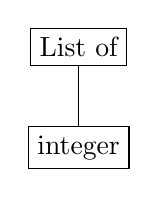
\begin{tikzpicture}
		\node[align=center, draw] (root)
		  {List of}
		;
		
    \draw (root) -- +(0, -1) node[draw, anchor=north](q) {integer};
		%  +(0,-1) 
\end{tikzpicture}
\begin{center}
(C) List of Temperatures
\end{center}

\end{center}
\caption{Weather Data Maps}
\label{data-maps-weather}
\end{figure}

Finding data sources can be a challenging task.
A component of my research plan is to publish best practices and techniques for finding, organizing, and exposing datasets.
The CORGIS collection already contains three dozen libraries, covering areas as diverse as international studies, nutrition, and social media platforms.
Some datasets were chosen because they were low-hanging fruit -- extensively documented, freely available, and well-supported. 
However, other datasets were driven by students' needs; in the two semesters that the course has been offered, two dozen new datasets have been created on demand.
The rapid turn-around time required has given new insight into the process of data mangling, although I am still exploring methods.
A massive part of my proposed work is to solidify and publish these techniques into a full paper.
